\section{Oefeningen}
\subsection{Opgaven logica}
\begin{enumerate}
\item Een persoon neemt bij het eten volgende regel in acht:
Als hij koffie drinkt, dan neemt hij geen melk.
Hij eet beschuiten enkel en alleen als hij melk drinkt.
Hij neemt geen soep samen met beschuiten.
Zoek de waarheidstabel van de logische uitdrukking die hierbij hoort. 
Als je weet dat hij koffie drinkt, kan je dan besluiten dat hij ook soep drinkt?
\item Vereenvoudig met behulp van een waarheidstabel:$(p \of q) \alsdan (p \en q)$
\item \begin{enumerate}
\item Bewijs dat $p \asa q$ equivalent is met $(p \alsdan q) \en (q \alsdan p)$
\item Bewijs dat $p \alsdan q$ equivalent is met $\niet p \of q$
\end{enumerate}
\item We definieerden voegwoorden (zie theorie) steeds via een tabel als volgt (tabel~\ref{tbl:voegwo}):
\begin{table}[htb]
  \centering
\begin{tabular}{|c|c|c|}
\hline
p  & q  & \mbox{formule met voegwoord} \\ \hline \hline
0  & 0   & \ldots \\
0  & 1 & \ldots \\ 
1  & 0 & \ldots \\
1  & 1 & \ldots \\
\hline
\end{tabular}
  \caption{Waarheidstabel voor twee veranderlijken}\label{tbl:voegwo}
\end{table}
Op de plaats van de `\ldots' komt een $0$ of een $1$ te staan. Hoeveel verschillende `derde' kolommen kan je zo maken? Schrijf op een systematische manier alle mogelijkheden in tabel~\ref{tbl:systematisch}. Duid alle bekende voegwoorden aan en probeer iets te bedenken voor de resterende mogelijkheden (er zijn soms meerdere antwoorden mogelijk).
\begin{table}[htb]
  \centering
\begin{tabular}{|c|c|p{0.3cm}|p{0.3cm}|p{0.3cm}|p{0.3cm}|p{0.3cm}|p{0.3cm}|p{0.3cm}|p{0.3cm}|p{0.3cm}|p{0.3cm}|p{0.3cm}|p{0.3cm}|p{0.3cm}|p{0.3cm}|p{0.3cm}|p{0.3cm}|}
\hline
p  & q  & & & & & & & & & & & & & & \\ \hline \hline
0  & 0   & & & & & & & & & & & & & &  \\
0  & 1 & & & & & & & & & & & & & &  \\ 
1  & 0 & & & & & & & & & & & & & &  \\
1  & 1 & & & & & & & & & & & & & &  \\
\hline
\end{tabular}
  \caption{Alle mogelijke combinaties voor de derde kolom}\label{tbl:systematisch}
\end{table}
\item Stel de waarheidstabel voor volgende samengestelde uitspraken op. Geef ook aan of de uitspraak een tautologie of een contradictie is.
\begin{enumerate}
\item $(p \of (q \en r)) \en \niet(p \en (q \of r))$
\item $\niet(p \of q) \en (p \en q)$
\item $(p \en \niet q) \of (\niet p \of q)$
\item $(p \of q \alsdan r) \asa (p\alsdan r) \en (q\alsdan r)$
\end{enumerate}
\item Er werd een moord gepleegd. Sherlock Holmes komt ter plaatse en stelt volgende zaken vast:
De kok of de butler waren in de keuken.
De kok was in de keuken of in de eetkamer.
Als de butler een sigaar rookte, dan was hij niet in de keuken.
Als de kok niet in de eetkamer was, dan rookte de butler geen sigaar.
Welk eenvoudig besluit kan je trekken (gebruik een waarheidstabel).
\item Bob, Jan en Koen worden verdacht van belastingontduiking. Elk van hen getuigt als volgt:
Bob: `Jan is schuldig en Koen is onschuldig'.
Jan: `Als Bob schuldig is, dan is Koen het ook'.
Koen: `Ik ben onschuldig, maar tenminste \'{e}\'{e}n van de anderen is schuldig'.
De elementaire uitspraken die erin voorkomen zijn `een persoon is schuldig of onschuldig'. We spreken af dat de proposities $b$, $j$ en $k$ respectievelijk betekenen `Bob is onschuldig', `Jan is onschuldig', en `Koen is onschuldig'.
\begin{enumerate}
\item Stel de waarheidstafels op van elk van deze getuigenissen. Plaats ze naast elkaar. Zet eerst de getuigenissen om in logische formules.
\item Is er \'{e}\'{e}n situatie waarin alle getuigenissen samen waar zijn? (Dit noemt men \emph{consistent}). Zo ja, wie is er dan schuldig?
\item Als we veronderstellen dat iedereen onschuldig is, wie liegt er dan?
\item Als we van de simpele redenering uitgaan dat elke schuldige liegt en elke onschuldige de waarheid spreekt, wie is dan schuldig of onschuldig?
\end{enumerate}
\end{enumerate}


\subsection{Opgaven Boolse Algebra}

\begin{enumerate}
\item Gegeven is volgend elektronisch schema (figuur~\ref{fig:schema1}). Geef de schakelfunctie waarvan dit schema de letterlijke weergave is. Vind vervolgens een eenvoudiger schema dat equivalent is (maar minder poorten bevat) met het oorspronkelijk schema door toepassen van regels van de Boolse Algebra.
\begin{figure}[htbp]
\begin{center}
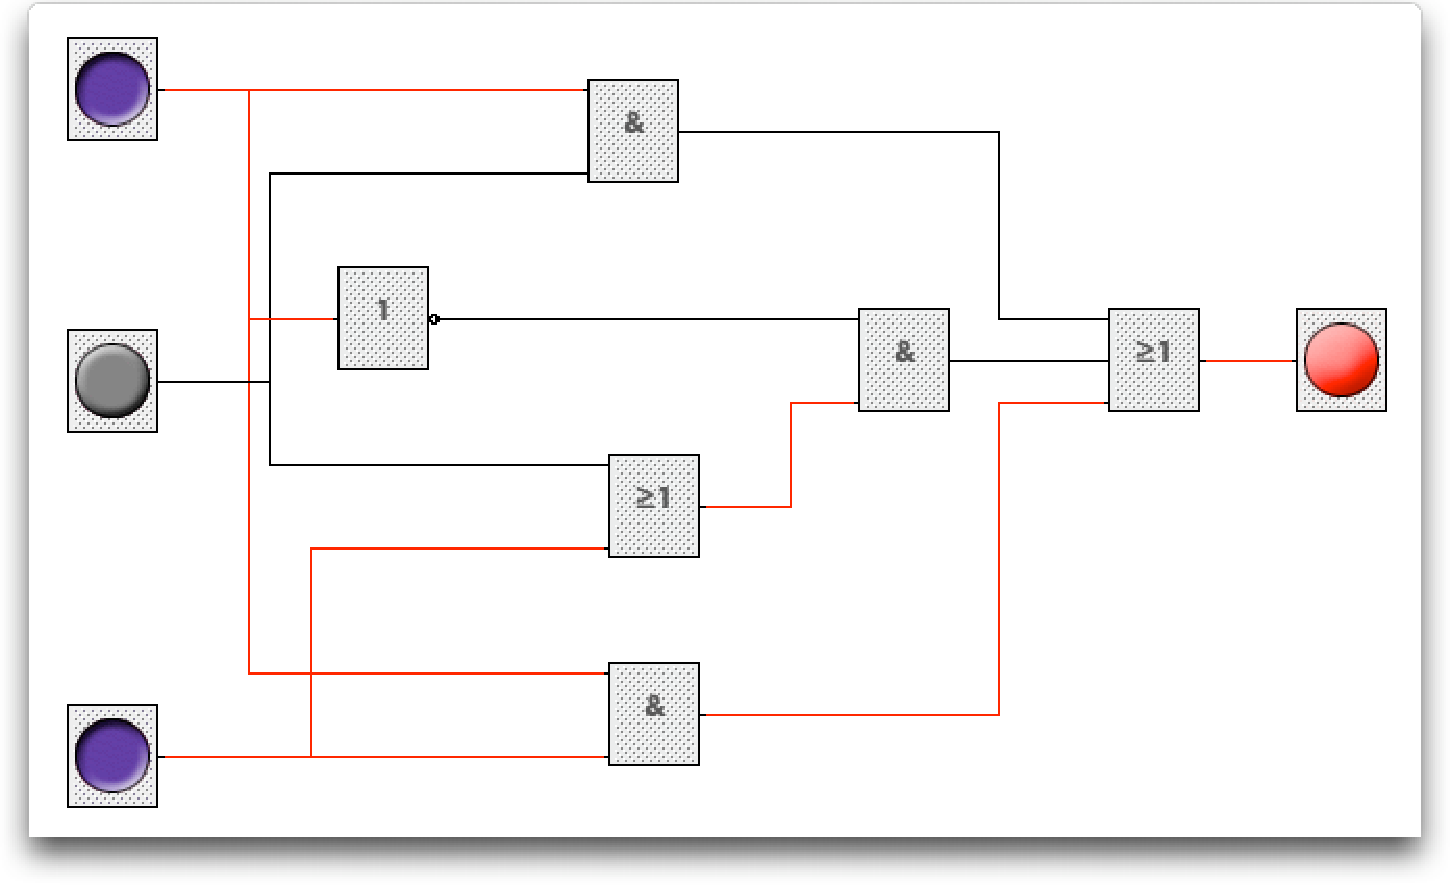
\includegraphics[width=\textwidth]{figuren/boole/el_schema1.pdf}
\caption{Schakeling met drie ingangen}
\label{fig:schema1}
\end{center}
\end{figure}
\item Werk volgende boolse functies om tot een standaard som van producten en standaard product van sommen. Welke distributiviteit moet je gebruiken?
\begin{enumerate}
\item $a(x,y,z)=x\cdot \overline{y+z} + y\cdot z$
\item $b(x,y,z)=x\cdot \overline{y\cdot z} + \overline{x}\cdot \overline{y}$
\item $c(x,y,z)=\overline{x}\cdot \overline{x\cdot \overline{z}}\cdot \overline{y} + z$
\item $d(x,y,z,t)=\overline{x+\overline{y+t}} + \overline{t\cdot x+z\cdot y}$
\end{enumerate}

\item In een kamer hangt 1 lamp. Deze lamp kan d.m.v.\ 3 schakelaars bediend worden. Met elke schakelaar kan je de brandende lamp doven, of de gedoofde lamp terug aansteken. Veronderstel dat als de drie schakelaars tegelijk op $0$ staan, de lamp niet brandt. Stel een waarheidstabel op voor de functie die het al of niet branden van de lamp beschrijft in functie van de stand van de drie schakelaars. Schrijf de conjunctieve en de disjunctieve normaalvormen die overeenkomen met deze tabel.
\item Volgende schakelfunctie wordt enkel gegeven door haar waarheidstabel (tabel~\ref{tbl:oefwaarh}). Je kent er m.a.w.\ geen voorschrift van. Schrijf de conjunctieve en de disjunctieve normaalvormen die overeenkomen met deze tabel.
\begin{table}[htb]
  \centering
\begin{tabular}{|cccc|c|}
\hline
  $a$ & $b$ & $c$ & $d$ & $f(a,b,c,d)$ \\ \hline \hline
  0 & 0 & 0 & 0 & 0 \\
  0 & 0 & 0 & 1 & 0 \\
  0 & 0 & 1 & 0 & 1 \\ 
  0 & 0 & 1 & 1 & 1 \\
  0 & 1 & 0 & 0 & 1 \\
  0 & 1 & 0 & 1 & 0 \\
  0 & 1 & 1 & 0 & 0 \\
  0 & 1 & 1 & 1 & 0 \\
  1 & 0 & 0 & 0 & 1 \\
  1 & 0 & 0 & 1 & 0 \\
  1 & 0 & 1 & 0 & 1 \\
  1 & 0 & 1 & 1 & 0 \\
  1 & 1 & 0 & 0 & 1 \\
  1 & 1 & 0 & 1 & 0 \\
  1 & 1 & 1 & 0 & 1 \\
  1 & 1 & 1 & 1 & 1 \\
\hline
\end{tabular}
  \caption{Functie gegeven door waarheidstabel}\label{tbl:oefwaarh}
\end{table}

\item Herneem de oefeningen uit oefening 2. Hoe kan je controleren of je rekenwerk bij deze oefeningen correct gebeurd is? Voer de controle uit.
\end{enumerate}


\subsection{Vereenvoudigen via Karnaugh-afbeeldingen}
\begin{enumerate}
\item Schrijf volgende functies voluit (als som van producten of product van sommen). Probeer ze vervolgens zoveel mogelijk te vereenvoudigen (als som van producten).
\begin{enumerate}
\item $f(x, y, z) = \prod M(0, 1, 2, 6)$
\item $f(A, B, C, D) = \sum m(1, 5, 6, 7, 11, 12, 13, 15)$
\item $f(A, B, C, D) = \prod M(7, 9, 13)$
\item $f(A, B, C, D) = \sum m(0, 1, 2, 5, 8, 10)$
\end{enumerate}

\item Volgende functie is gegeven via een waarheidstabel (tabel~\ref{tbl:f2}). Maak een realisatie met zo weinig mogelijk poorten. Teken vervolgens de schakeling.
\begin{table}[htb]
  \centering
\begin{tabular}{|ccc|c|}
\hline
$x$  & $y$ & $z$ & $f(x,y,z)$ \\ \hline \hline
0 & 0  & 0 & 1 \\
0 & 0  & 1 & 1\\ 
0 & 1  & 0 & 0\\
0 & 1  & 1 & 0\\
1 & 0  & 0 & 0 \\
1 & 0  & 1 & 1\\ 
1 & 1  & 0 & 1\\
1 & 1  & 1 & 1\\

\hline
\end{tabular}
  \caption{Functie $f$ gegeven door waarheidstabel}\label{tbl:f2}
\end{table}

\item We kunnen ook een functie minimaliseren tot een \emph{product van sommen}. Deze techniek werkt als volgt. Schrijf alleen de vakjes met een 0 in een Karnaugh-afbeelding (de vakjes waar een 1 moet komen laat je leeg). Probeer nu te vereenvoudigen door naburige vakjes met een 0 erin samen te nemen. Elke groep van nullen die je kan samennemen schrijf je nu als een som, waarbij de variabelen net het complement zijn van wat er zou komen als je enen samenvoegt bij het minimaliseren tot een som van producten (dit is een toepassing van dualiteit!). Volgend voorbeeld maakt dit duidelijk:

Gegeven $f(A, B, C) = \prod M(3, 6, 7)$. De overeenkomstige Karnaugh-afbeelding bevat 3 nullen en 5 enen. Normaal gezien bekijken we alleen de 1 in een Karnaugh-afbeelding. Voor \emph{product van sommen}-vorm werken we alleen met de vakjes met een 0. Je vindt figuur~\ref{fig:Karn1}.
\begin{figure}[htb]
\begin{center}
\karnaughmap{3}{$f(a,b,c):$}{{$a$}{$b$}{$c$}}{11101100}%
{%
\put(3,0.5){\oval(1.8,0.8)}
}
\caption{Karnaugh-afbeelding van de schakelfunctie $f$}
\label{fig:Karn1}
\end{center}
\end{figure}


Als je samenneemt zoals hierboven, welke veranderlijke verdwijnt dan? Waarom? 
Er blijft dus een som van twee letters over (met of zonder complementstreepje erboven). We redeneren nu als volgt: de functiewaarde moet 0 worden voor de input die hoort bij die samengenomen vakjes, dus voor $A = 1$ en $B = 1$. We vinden bijgevolg $(\overline{A}+\overline{B})$. Groepeer nu de overblijvende 0 met een naburig vakje (ev.\ reeds gebruikt!), en herhaal de stappen. Je vindt: $f(A, B, C) = (\overline{A}+\overline{B})\cdot (\overline{B}+\overline{C})$

Vind nu een minimale realisatie voor volgende functies als \emph{product van sommen}. Geef ook een realisatie als \emph{som van producten}, en ga na welke vorm het eenvoudigst is.
\begin{enumerate}
\item $f (A, B, C, D) = \sum m(0, 2, 10, 11, 12, 14)$
\item $f (A, B, C, D) = \prod M(1, 3, 4, 5, 6, 7, 9, 10, 11, 14, 15)$
\end{enumerate}

\item Probeer de functie uit het lampenprobleem (oef 3 Boolse Algebra) d.m.v. een Karnaugh-afbeelding te minimaliseren.

\item Een schakeling krijgt twee 2-bit binaire getallen als input, nl. getal $A = A_{1}A_{0}$, en getal $B = B_{1}B_{0}$. Ontwerp een minimale som van producten realisatie als de schakeling alleen een output 1 mag geven als $A$ groter is dan $B$.

\end{enumerate}
